\documentclass[a4paper]{article}
\usepackage[letterpaper,top=2cm,bottom=2cm,left=3cm,right=3cm,marginparwidth=1.75cm]{geometry}
\usepackage[colorlinks=true, allcolors=blue]{hyperref}

\usepackage{wrapfig}
\usepackage{amsthm}
\usepackage{hyperref}
\usepackage{graphicx}
\usepackage{amsfonts}

\title{Homework 2: Krylov Methods}
\author{Patryk Drozd}
\begin{document}
\date{}
\maketitle

\section*{2}
	Structure

\section*{2.1}

\section*{2.2}
	
	For the serial implementation of GMRES in python I chose to follow Algorithm 6.9 from 
	\textit{Iterative Methods for Sparse Linear Systems by Yousef Saad}. For solving the 
	minimization problem in line 12 I used a least squares solver taken form the numpy 
	library.

	Figure \ref{fig:q2_fig} shows for $n = 8, 16, 32, 64, 128, 256$ the serial gmres function run
	for $m = n/2$ iterations. In this plot we can see that residual of the 

	$$\frac{||r_k||_2}{||b||_2} \propto n^{-a}$$


	\begin{figure}[h!]
	    \centering
    	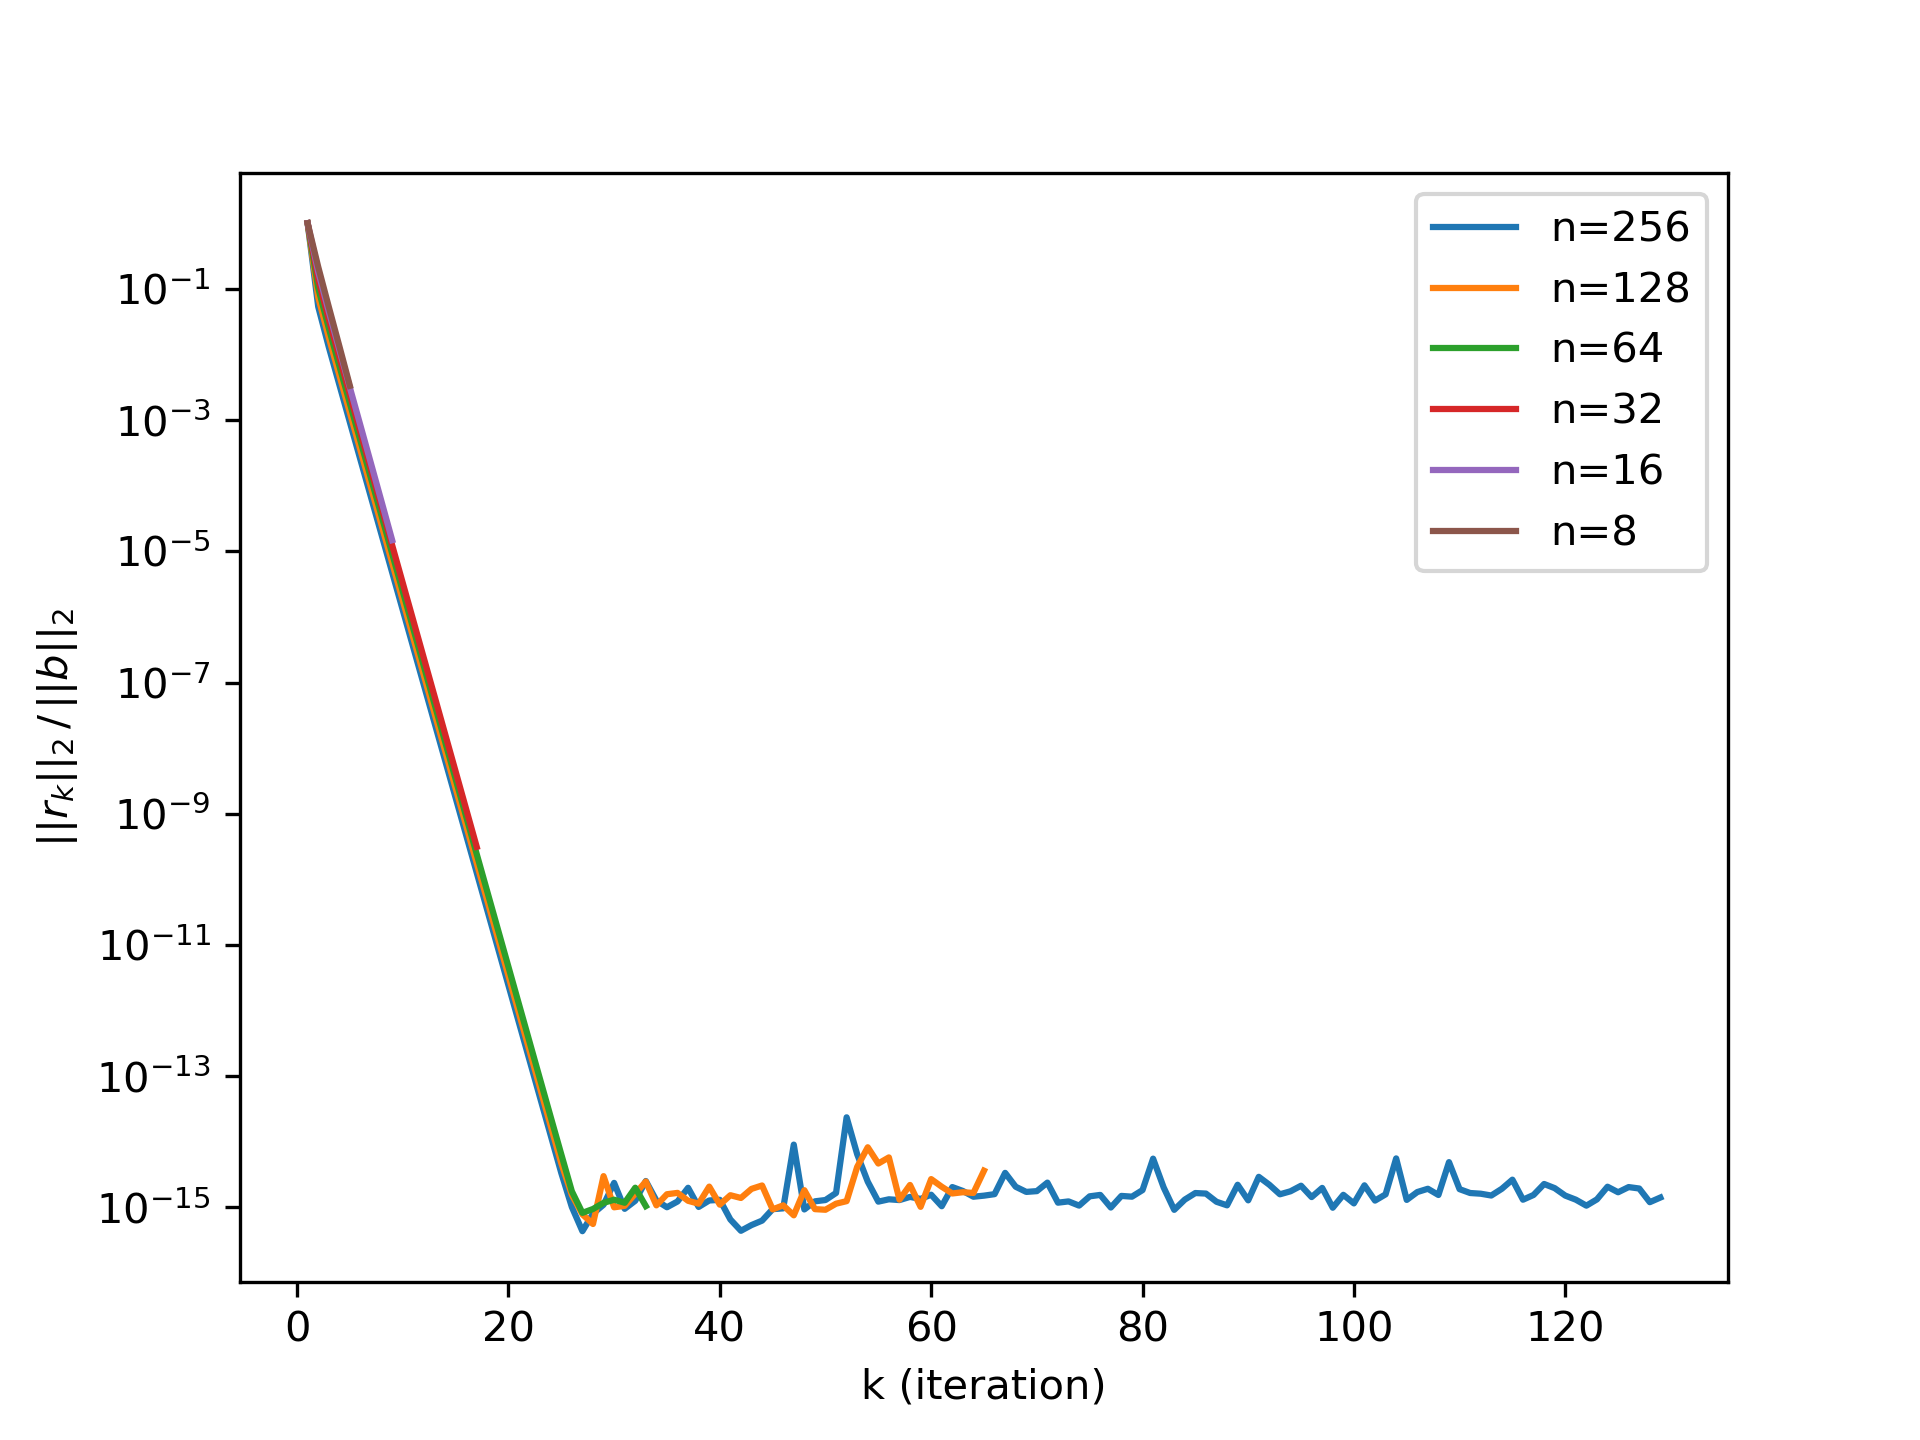
\includegraphics[width=.8\linewidth]{./q2_fig.png}
    	\label{fig:q2_fig}
	\end{figure}

\section*{2.3}
		


\bibliographystyle{plain} 
\bibliography{refs} 

\end{document}



